\chapter{MIMO Communication Performance Evaluation}

Having characterized the antenna element and the metasurface transmitarray lens individually in the preceding chapter, this chapter evaluates their system-level communication performance in a multi-antenna link. The evaluation is carried out with Sionna-RT, which reconstructs the wireless channel from the propagation environment and imported antenna far-field patterns. Two complementary controlled protocols are used. First, linear and half-circular transmitter trajectories provide paired lens-assisted and without-lens comparisons at identical waypoints for the $9\times9$ configuration. Second, lens-assisted $3\times3$, $5\times5$, and $9\times9$ configurations traverse the same linear trajectory to characterize higher-order scaling. The first protocol compares complete RX placement-and-pattern designs, whereas the second shows how absolute and normalized channel metrics evolve when array order, total radiated power, aperture, and RX angular sampling change together.

\section{Comparison of Different Antenna Placements}\label{sec:comparison-antenna-placements}

This section compares two complete nine-branch receiver (RX) configurations using the four ISO-TX simulation datasets in the available analysis package, which covers Sections~1--14 of the source workflow. In every case, a nine-element isotropic transmitter (TX) array radiates simultaneously while its center follows either a linear or half-circular trajectory. The lens-assisted and without-lens cases reuse the same TX array and waypoint sequence within each trajectory, so the within-trajectory comparison is paired with respect to TX motion.

Under the equal-weight aggregation used in these simulations, the without-lens baseline provides the higher median link capacity and constructed MIMO capacity, as well as a higher effective rank, on both trajectories. The lens-assisted configuration instead produces a much wider spread across its angle-specific RX branches and higher typical-block decorrelation. These results characterize the complete RX designs rather than the lens alone: the lens branches occupy a compact focal arc and use different angle-specific far-field patterns, whereas the baseline branches form a coplanar array and use the same $0^\circ$ patch pattern. Placement and imported pattern therefore change together.

\subsection{Simulation Configuration and Paired Trajectories}

The common simulation settings are listed in Table~\ref{tab:iso9x9-simulation-setup}. The linear path contains 21 waypoints along a 19~m line. The half-circular path contains 37 waypoints on a 9~m-radius semicircle, giving a path length of 28.27~m. Each waypoint is sampled over 16 mobility time steps. Consequently, the lens and without-lens cases contain 189 waypoint--RX observations each on the linear path and 333 each on the half-circular path.

\begin{table}[htbp]
    \centering
    \caption{Common simulation configuration for the paired 9-ISO-TX comparison.}
    \label{tab:iso9x9-simulation-setup}
    \footnotesize
    \renewcommand{\arraystretch}{1.15}
    \begin{tabularx}{\linewidth}{@{}>{\raggedright\arraybackslash}p{0.31\linewidth} >{\raggedright\arraybackslash}X@{}}
        \toprule
        \textbf{Parameter} & \textbf{Value} \\
        \midrule
        Room; carrier frequency & $20\,\text{m}\times20\,\text{m}\times3\,\text{m}$; 38~GHz \\
        Bandwidth; frequency sampling & 400~MHz; 401 frequency bins \\
        TX configuration & Nine simultaneous isotropic elements; 10~dBm per element \\
        Noise model & 7~dB noise figure at 290~K \\
        Mobility sampling & 1~kHz; 16 time steps per waypoint; 1~m/s \\
        Ray-tracing samples & 100{,}000 path samples per source \\
        Linear trajectory & 21 waypoints; 19.00~m \\
        Half-circular trajectory & 37 waypoints; 9~m radius; 28.27~m \\
        \bottomrule
    \end{tabularx}
\end{table}

Figure~\ref{fig:iso9x9-trajectory-geometry} shows that both RX clusters have nearly the same room-scale reference location near $(-9,0,2)$~m and that the TX trajectories are identical across the two configurations. Locally, however, the baseline elements lie on a 44.24~mm straight line, while the lens-assisted points follow a compact focal arc spanning approximately 29.44~mm in the $y$ direction. The latter use nine lens patterns from $+60^\circ$ to $-60^\circ$ in $15^\circ$ increments. Thus, matching branch indices identify ordinal design cases rather than co-located antenna elements.

\clearpage
\begin{figure}[p]
    \centering
    
\includegraphics[width=\linewidth]{Images/Analisis_v4_ISO_TX_Lens_vs_WithoutLens_Linear_HalfCircular_9x9/figures_matlab/01_geometry_and_arrays_matlab.png}
    \caption{Paired TX trajectories and local array geometry for the 9-ISO-TX comparison. The linear and half-circular waypoint sequences are identical for the two RX designs, but the baseline uses a coplanar RX array whereas the lens-assisted configuration uses a compact focal-arc arrangement with angle-specific patterns.}
    \label{fig:iso9x9-trajectory-geometry}
\end{figure}
\clearpage

\subsection{Evaluation Metrics and Aggregation}

For each active RX branch, the nine isotropic TX contributions are combined non-coherently in the link budget. If $H_i(f)$ is the channel response of TX element $i$ at frequency $f$, the received power, SNR, and equivalent-SISO Shannon capacity are
\begin{equation}
    \begin{aligned}
        P_\mathrm{RX}(f)&=P_\mathrm{TX}\sum_{i=1}^{9}|H_i(f)|^2,
        &\gamma(f)&=\frac{P_\mathrm{RX}(f)}{kTB\,10^{\mathrm{NF}/10}},\\
        C_\mathrm{link}&=\frac{1}{N_f}\sum_f\log_2\!\left(1+\gamma(f)\right).
    \end{aligned}
    \label{eq:iso9x9-link-capacity}
\end{equation}
This link-budget capacity represents nine TX elements feeding one active RX branch; it is distinct from the constructed $9\times9$ MIMO capacity described below.

At every waypoint, the nine sequential $9\times1$ RX simulations are stacked to form a constructed channel matrix $\mathbf{H}(f)$. With singular values $\sigma_1(f)\geq\cdots\geq\sigma_9(f)$, the condition number and effective rank are
\begin{equation}
    \kappa(f)=\frac{\sigma_1(f)}{\sigma_9(f)},
    \qquad
    r_\mathrm{eff}(f)=\exp\!\left[-\sum_{i=1}^{9}p_i(f)\ln p_i(f)\right],
    \qquad
    p_i(f)=\frac{\sigma_i^2(f)}{\sum_{j=1}^{9}\sigma_j^2(f)}.
    \label{eq:mc9x9-condrank}
\end{equation}
The equal-power ideal capacity of this constructed matrix is
\begin{equation}
    C_\mathrm{MIMO}(\gamma)=\mathbb{E}_f\!\left[
    \sum_{i=1}^{9}\log_2\!\left(1+\frac{\gamma}{N_t}\sigma_i^2(f)\right)
    \right],
    \qquad N_t=9,
    \label{eq:mc9x9-mimocapacity}
\end{equation}
and is evaluated at 10~dB after the fixed-SNR channel normalization used by the source workflow. It is therefore a channel-structure metric rather than an absolute link-budget quantity and is not directly comparable with $C_\mathrm{link}$ in Equation~\ref{eq:iso9x9-link-capacity}. A smaller condition number and a larger effective rank are favorable. Because the nine RX channels are simulated sequentially rather than measured simultaneously, these quantities diagnose spatial structure and diversity potential; they do not represent the directly realizable capacity of a single nine-port receiver.

Spatial decorrelation is evaluated separately for the center TX element (index~4) across the nine RX responses. Let $h_i[n]$ and $h_j[n]$ be complex channel-frequency-response samples for RX branches $i$ and $j$. Their normalized correlation and decorrelation are
\begin{equation}
    \rho_{ij}=\frac{\sum_n h_i[n]h_j^*[n]}
    {\sqrt{\left(\sum_n|h_i[n]|^2\right)\left(\sum_n|h_j[n]|^2\right)}},
    \qquad D_{ij}=1-|\rho_{ij}|.
    \label{eq:iso9x9-spatial-correlation}
\end{equation}
Two aggregation scopes are retained. The global pooled value applies Equation~\ref{eq:iso9x9-spatial-correlation} after concatenating all waypoint, time, and frequency samples. The robust value first evaluates block-level correlation and then takes its median,
\begin{equation}
    D_{ij}^{\mathrm{med}}=1-\operatorname{median}_{w,t}\!\left|\rho_{ij}^{(w,t)}\right|.
    \label{eq:iso9x9-median-decorrelation}
\end{equation}
The along-path pooled curves instead pool samples separately within each waypoint. These three summaries have different weighting and must not be treated as interchangeable. The unnormalized difference power, $Q_{ij}^{\mathrm{raw}}=N^{-1}\sum_n|h_i[n]-h_j[n]|^2$, is also retained to show absolute channel-power differences, but it cannot by itself establish channel independence.

\subsection{Static Snapshot Characterization}

The static snapshot in Figure~\ref{fig:iso9x9-static-rx} illustrates the main design contrast. The without-lens combined gain is almost invariant across the nine RX branches, ranging only from approximately $-73.12$ to $-73.05$~dB. The angle-specific lens branches span approximately $-72.04$ to $-68.03$~dB and are stronger at all nine ordinal indices in this snapshot; their median is $-70.63$~dB, compared with $-73.10$~dB without the lens. This wide range confirms strong angular selectivity, but it does not imply that all lens branches retain the same advantage as the TX moves. The normalized per-branch capacities at 10~dB remain close to 3.4~bit/s/Hz for both designs because this particular snapshot comparison normalizes the operating SNR.

\begin{figure}[htbp]
    \centering
    
\includegraphics[width=\linewidth]{Images/Analisis_v4_ISO_TX_Lens_vs_WithoutLens_Linear_HalfCircular_9x9/figures_matlab/02_static_rx_scenario_comparison_matlab.png}
    \caption{Static comparison of combined gain, TX-branch correlation, and normalized capacity for the nine RX design cases. Matching indices are ordinal design pairs rather than co-located elements.}
    \label{fig:iso9x9-static-rx}
\end{figure}

The constructed static matrix in Figure~\ref{fig:iso9x9-static-mimo} gives a similarly mixed result. The lens lowers the snapshot condition number from 30.60 to 25.10~dB, but the effective rank decreases from 5.42 to 5.12 and capacity at 10~dB changes only from 24.06 to 23.88~bit/s/Hz. The mean off-diagonal RX correlation also increases from 0.22 to 0.27. Consequently, a lower condition number alone is insufficient evidence of improved multiplexing; the singular-value distribution, correlation, and capacity must be considered together.

\begin{figure}[htbp]
    \centering
    
\includegraphics[width=\linewidth]{Images/Analisis_v4_ISO_TX_Lens_vs_WithoutLens_Linear_HalfCircular_9x9/figures_matlab/03_static_mimo_comparison_matlab.png}
    \caption{Constructed $9\times9$ MIMO metrics at the static snapshot. The matrix combines nine sequential $9\times1$ RX simulations and is used as a channel-structure diagnostic.}
    \label{fig:iso9x9-static-mimo}
\end{figure}

\subsection{Aggregate and Along-Trajectory Link Performance}

Table~\ref{tab:iso9x9-aggregate-results} and Figure~\ref{fig:iso9x9-aggregate} summarize the main trajectory results. Medians are computed from the complete waypoint--RX population for each configuration. For both paths, the equal-weight ensemble favors the without-lens baseline in channel magnitude and link capacity. On the linear path, the lens decreases median channel magnitude by 6.87~dB and link capacity by 1.81~bit/s/Hz, or 25.86\%. On the half-circular path, the corresponding decreases are 3.64~dB and 1.03~bit/s/Hz, or 17.05\%.

\begin{table}[htbp]
    \centering
    \caption{Aggregate link, constructed-MIMO, and spatial-decorrelation metrics for the paired trajectories. Both capacity columns are in bit/s/Hz. $D_\mathrm{global}$ is pooled over all realizations; $D_\mathrm{med}$ is the median block-level decorrelation.}
    \label{tab:iso9x9-aggregate-results}
    \scriptsize
    \renewcommand{\arraystretch}{1.15}
    \begin{tabularx}{\linewidth}{@{}>{\raggedright\arraybackslash}p{0.13\linewidth} >{\raggedright\arraybackslash}p{0.14\linewidth} *{7}{>{\centering\arraybackslash}X}@{}}
        \toprule
        \textbf{Path} & \textbf{RX design} & \textbf{$|H|_\mathrm{med}$ (dB)} & \textbf{$C_\mathrm{link}$} & \textbf{$\kappa_\mathrm{med}$ (dB)} & \textbf{$r_\mathrm{eff,med}$} & \textbf{$C_\mathrm{MIMO}$} & \textbf{$D_\mathrm{global}$} & \textbf{$D_\mathrm{med}$} \\
        \midrule
        Linear & Without lens & $-79.78$ & $7.00$ & $43.56$ & $3.160$ & $17.20$ & $0.9493$ & $0.0885$ \\
        Linear & Lens & $-86.65$ & $5.19$ & $42.88$ & $2.043$ & $14.56$ & $0.8570$ & $0.4876$ \\
        Half-circular & Without lens & $-83.60$ & $6.04$ & $39.90$ & $3.965$ & $19.99$ & $0.9236$ & $0.2109$ \\
        Half-circular & Lens & $-87.24$ & $5.01$ & $40.81$ & $2.391$ & $16.17$ & $0.8634$ & $0.5840$ \\
        \bottomrule
    \end{tabularx}
\end{table}

\clearpage
\begin{figure}[p]
    \centering
    
\includegraphics[width=\linewidth]{Images/Analisis_v4_ISO_TX_Lens_vs_WithoutLens_Linear_HalfCircular_9x9/figures_matlab/08_aggregate_comparison_matlab.png}
    \caption{Aggregate comparison of the lens-assisted and without-lens RX designs for nine isotropic TX elements. Channel magnitude and link capacity are medians over waypoint--RX observations; MIMO metrics use the constructed $9\times9$ channel; spatial decorrelation is reported at both global-pooled and median-block scopes.}
    \label{fig:iso9x9-aggregate}
\end{figure}
\clearpage

Figure~\ref{fig:iso9x9-link-trajectory} shows that the mean without-lens SNR and capacity remain above the lens mean at every sampled waypoint on both paths. The shaded lens region is the minimum-to-maximum range across the nine RX cases, not a confidence interval. Its width shows that individual angle-specific branches can be much stronger or weaker than the ensemble mean. All four configurations record 0\% outage at the 1~bit/s/Hz threshold. This threshold is therefore saturated and cannot distinguish reliability; higher thresholds or capacity percentiles are required for a useful outage comparison.

\clearpage
\begin{figure}[p]
    \centering
    
\includegraphics[width=\linewidth]{Images/Analisis_v4_ISO_TX_Lens_vs_WithoutLens_Linear_HalfCircular_9x9/figures_matlab/04_channel_metrics_along_trajectory_matlab.png}
    \caption{Mean SNR and equivalent-SISO link capacity along the linear and half-circular trajectories. Lines are means across the nine RX cases, and the shaded lens bands are the corresponding minimum-to-maximum ranges. The horizontal capacity reference is the 1~bit/s/Hz outage threshold.}
    \label{fig:iso9x9-link-trajectory}
\end{figure}
\clearpage

\subsection{Constructed MIMO Performance Along the Trajectories}

The lens-assisted design also produces lower median constructed-MIMO capacity and effective rank on both paths. For the linear trajectory, median capacity at 10~dB falls from 17.20 to 14.56~bit/s/Hz and effective rank from 3.160 to 2.043. The median condition number improves only slightly, from 43.56 to 42.88~dB. For the half-circular trajectory, capacity falls from 19.99 to 16.17~bit/s/Hz, effective rank from 3.965 to 2.391, and the condition number worsens slightly from 39.90 to 40.81~dB. Thus, neither a small condition-number change nor local beam separation compensates for the lower effective rank under the present construction.

Figure~\ref{fig:iso9x9-mimo-trajectory} also reveals a sharp symmetry-related impairment near the midpoint of the linear path at 9.5~m: the condition number reaches 89.51~dB without the lens and 71.89~dB with the lens, while the corresponding MIMO capacities fall to 8.06 and 7.84~bit/s/Hz. The half-circular trajectory avoids such a severe isolated singularity and yields a higher median effective rank and MIMO capacity for both designs. This between-path difference is descriptive, however, because path shape, location, distance distribution, and waypoint count change together.

\clearpage
\begin{figure}[p]
    \centering
    
\includegraphics[width=\linewidth]{Images/Analisis_v4_ISO_TX_Lens_vs_WithoutLens_Linear_HalfCircular_9x9/figures_matlab/05_trajectory_mimo_metrics_matlab.png}
    \caption{Condition number, effective rank, and ideal capacity at 10~dB for the constructed $9\times9$ channel along the two trajectories. The linear midpoint produces a pronounced conditioning singularity in both configurations.}
    \label{fig:iso9x9-mimo-trajectory}
\end{figure}
\clearpage

\subsection{Spatial Decorrelation}

The spatial result depends strongly on aggregation scope. When all realizations are concatenated before normalization, global pooled decorrelation is higher without the lens: 0.9493 versus 0.8570 on the linear path and 0.9236 versus 0.8634 on the half-circular path. By contrast, the block-median decorrelation favors the lens by a wide margin, increasing from 0.0885 to 0.4876 on the linear path and from 0.2109 to 0.5840 on the half-circular path. The waypoint-level curves in Figure~\ref{fig:iso9x9-decorrelation} likewise favor the lens because pooling is performed separately within each waypoint rather than over the full trajectory. The mean waypoint-level values are 0.4934 with the lens versus 0.1135 without it on the linear path and 0.5881 versus 0.2152 on the half-circular path.

These findings are not contradictory. Global pooling is energy-weighted over the complete trajectory and measures the coherence of the concatenated response. Median-block and waypoint-level summaries give more comparable weight to local conditions and show that a typical lens block has more differentiated angle responses. In addition, these metrics use only the center TX element, so they should not be equated with the full constructed $9\times9$ singular-value metrics.

\begin{figure}[htbp]
    \centering
    
\includegraphics[width=\linewidth]{Images/Analisis_v4_ISO_TX_Lens_vs_WithoutLens_Linear_HalfCircular_9x9/figures_matlab/06_spatial_decorrelation_comparison_matlab.png}
    \caption{Waypoint-level pooled and median-based spatial decorrelation of the center TX element (index~4) across nine RX branches. Higher values indicate less-correlated local RX responses; these curves use a different aggregation scope from the global-pooled values in Table~\ref{tab:iso9x9-aggregate-results}.}
    \label{fig:iso9x9-decorrelation}
\end{figure}

The unnormalized difference power in Figure~\ref{fig:iso9x9-raw-difference} supplies amplitude context. Its ordering reflects both path loss and the RX-pattern gain, as well as the difference between channel responses. A larger value therefore cannot independently be interpreted as better decorrelation or higher multiplexing capacity.

\begin{figure}[htbp]
    \centering
    
\includegraphics[width=\linewidth]{Images/Analisis_v4_ISO_TX_Lens_vs_WithoutLens_Linear_HalfCircular_9x9/figures_matlab/07_raw_spatial_difference_power_matlab.png}
    \caption{Unnormalized spatial difference power along the linear and half-circular paths. Because the metric retains path loss and RX-pattern gain, it is interpreted only alongside the normalized decorrelation and link-budget metrics.}
    \label{fig:iso9x9-raw-difference}
\end{figure}

\subsection{Discussion and Limitations}

The combined results indicate a trade-off between uniform link performance and angular selectivity. The coplanar baseline applies the same patch pattern to nine closely spaced positions and therefore gives nearly uniform branch responses. The lens configuration instead samples nine directional patterns. Its median within-waypoint capacity spread is 6.78~bit/s/Hz on the linear path and 6.32~bit/s/Hz on the half-circular path, compared with only 0.02 and 0.05~bit/s/Hz, respectively, without the lens. At a given waypoint, one or more aligned beams can therefore be strong while non-aligned beams are weak; assigning equal statistical weight to all nine RX configurations lowers the reported lens median even though the local responses are more differentiated. The present result is specific to fixed, all-branch reporting and should not be generalized to a receiver that performs beam selection or combining. Such an operating strategy must be evaluated explicitly with a practical selection rule and switching overhead.

The half-circular path is more favorable to the constructed MIMO metrics for both RX designs because it avoids the severe midpoint singularity of the linear path and samples a broader sequence of relative angles. The available experiment does not isolate trajectory curvature as the cause, since the two paths also differ in position, distance distribution, length, and sample count. Only lens versus without-lens differences within the same trajectory are paired comparisons.

Several limitations constrain the inference. First, each constructed $9\times9$ matrix combines nine sequential $9\times1$ RX simulations, so simultaneous multiport reception, mutual coupling, and inter-port hardware phase consistency are not represented. Second, RX placement and far-field pattern differ together, preventing attribution to the lens material or focal displacement alone. Third, the results cover one scene, one ray-tracing realization set, and no multi-seed convergence or confidence-interval study. Fourth, 100{,}000 path samples per source were used, whereas the source workflow recommends 1{,}000{,}000 for a final high-accuracy run. Fifth, the along-path SNR and capacity curves were recovered from rounded notebook logs, although the headline medians use the higher-precision stored summaries. Finally, the exported package contains derived tables and figures rather than the complete complex CFR tensor, and it does not include the source notebooks or shared parser referenced by its provenance record. End-to-end regeneration and independent re-analysis beyond the reported metrics are therefore not possible from the present archive alone. The capacities are ideal Shannon or fixed-SNR channel measures and are not predictions of coded throughput.

\subsection{Summary of the Placement Comparison}

For nine simultaneous isotropic TX elements and equal statistical weighting of all nine RX configurations, the without-lens baseline provides stronger aggregate link and constructed-MIMO performance on the two evaluated trajectories. Relative to the baseline, the lens reduces median link capacity by 1.81~bit/s/Hz on the linear path and 1.03~bit/s/Hz on the half-circular path, while constructed-MIMO capacity decreases by 2.64 and 3.83~bit/s/Hz, respectively. The lens nevertheless produces substantially higher typical-block decorrelation, confirming stronger angular selectivity, while global pooled decorrelation remains higher without the lens. The half-circular path avoids the pronounced linear-path singularity and yields better constructed-MIMO statistics for both designs, but this is a descriptive path comparison. Future work should evaluate practical beam selection and combining, repeat the comparison at co-located RX coordinates, increase the path-sample count and random seeds, retain the full complex CFR tensor, and use informative outage thresholds or capacity percentiles.

\section{Higher-Order MIMO Systems}\label{sec:higher-order-mimo}

This section compares the complete lens-assisted $N\times N$ configurations for $N=3$, $5$, and $9$ using the controlled linear-trajectory outputs through Section~14 of the available analysis package. In every configuration, $N$ isotropic TX elements radiate simultaneously and the center of the TX array follows the same 21-waypoint path. The main result is a trade-off: increasing $N$ raises the link-budget capacity and fixed-SNR constructed-MIMO capacity, but the median condition number worsens and both effective rank per dimension and MIMO capacity per dimension decrease.

This trend is a configuration-level scaling result rather than a causal estimate of antenna order alone. The simulations apply 10~dBm to every TX element, keep the inter-element spacing fixed, and assign a different lens-angle grid to each order. Consequently, total radiated power, physical aperture, number of RX scenarios, and angular sampling all change with $N$.

\subsection{Simulation Configuration and Order Comparability}

The common environment is a $20\,\text{m}\times20\,\text{m}\times3\,\text{m}$ room at 38~GHz. The channel is sampled over 400~MHz using 401 frequency bins. The linear trajectory runs from $y=-9.5$~m to $y=+9.5$~m at $x=0$ and $z=2$~m, giving 21 waypoints and a total length of 19~m. Motion is evaluated at 1~m/s with 16 time samples per waypoint at 1~kHz. All configurations use a 7~dB receiver noise figure at 290~K and 100{,}000 path samples per source.

Table~\ref{tab:iso-order-simulation-setup} lists the quantities that change with order. The 0.45~m TX spacing expands the aperture from 0.90 to 3.60~m. Because the power is fixed at 10~dBm per TX, nominal total TX power rises by 4.77~dB from $N=3$ to $N=9$. The RX grids also differ; only the $0^\circ$ lens branch is common to all three configurations. The 63, 105, and 189 observations are waypoint--RX combinations, not independent Monte Carlo drops.

\begin{table}[htbp]
    \centering
    \caption{Order-dependent configuration for the controlled lens-assisted linear-trajectory comparison.}
    \label{tab:iso-order-simulation-setup}
    \footnotesize
    \renewcommand{\arraystretch}{1.15}
    \begin{tabularx}{\linewidth}{@{}>{\centering\arraybackslash}p{0.10\linewidth} >{\centering\arraybackslash}p{0.16\linewidth} >{\raggedright\arraybackslash}X >{\centering\arraybackslash}p{0.17\linewidth} >{\centering\arraybackslash}p{0.16\linewidth}@{}}
        \toprule
        \textbf{Order} & \textbf{TX aperture} & \textbf{RX lens-angle grid} & \textbf{Waypoint--RX observations} & \textbf{Nominal total TX power} \\
        \midrule
        $3\times3$ & 0.90~m & $-45^\circ,0^\circ,+45^\circ$ & 63 & 14.77~dBm \\
        $5\times5$ & 1.80~m & $-60^\circ$ to $+60^\circ$ in $30^\circ$ steps & 105 & 16.99~dBm \\
        $9\times9$ & 3.60~m & $-60^\circ$ to $+60^\circ$ in $15^\circ$ steps & 189 & 19.54~dBm \\
        \bottomrule
    \end{tabularx}
\end{table}

Figure~\ref{fig:iso-order-geometry} shows the common trajectory and the order-dependent TX and RX geometry. The increasingly dense lens grid does not compare the same set of physical RX branches at every order. Accordingly, all-order aggregate comparisons characterize each complete design, while the common $0^\circ$ branch is retained as a narrower sensitivity check.

\begin{figure}[htbp]
    \centering
    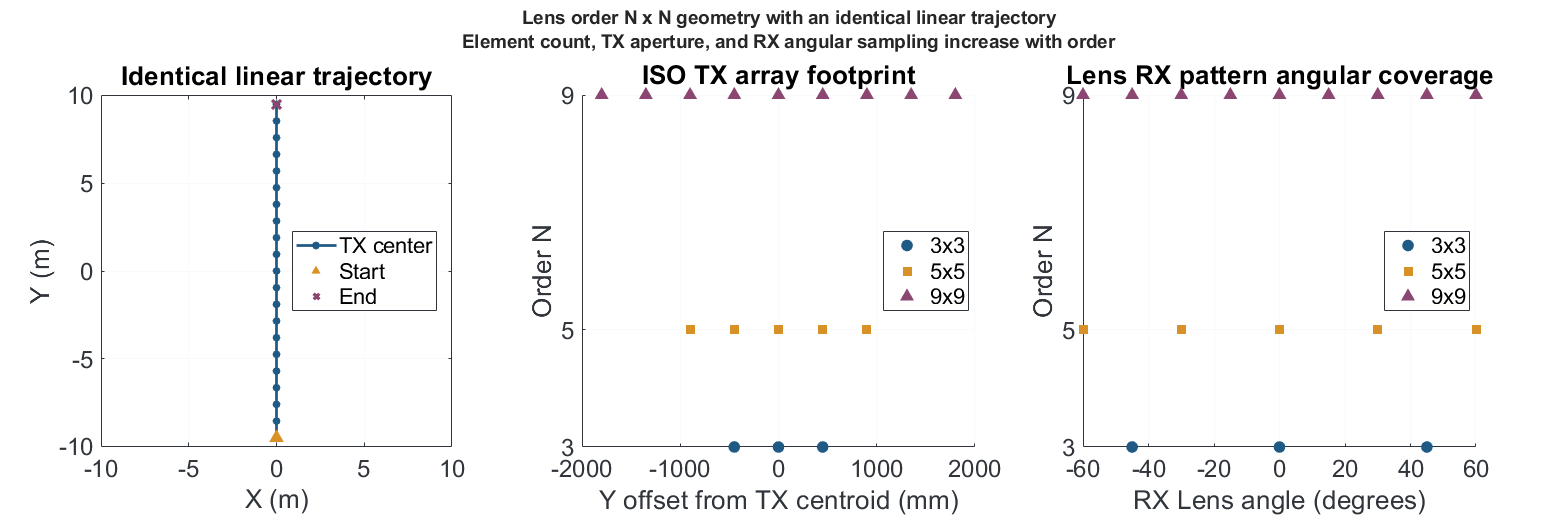
\includegraphics[width=\linewidth]{Images/Analisis_v4_ISO_TX_Lens_Order_3x3_5x5_9x9_Linear/figures_matlab/01_geometry_order_comparison_matlab.png}
    \caption{Common linear TX trajectory and order-dependent TX aperture and RX lens-angle grids for the $3\times3$, $5\times5$, and $9\times9$ configurations.}
    \label{fig:iso-order-geometry}
\end{figure}

\subsection{Metrics and Normalization}

The link-budget capacity follows Equation~\ref{eq:iso9x9-link-capacity}, with the TX summation limit changed from 9 to $N$. It combines the received power from all simultaneously active TX elements at one active RX branch. The aggregate link statistics pool all waypoint--RX observations within an order. They therefore include both the growing total TX power and the different RX-angle populations.

For the spatial analysis, the $N$ sequential $N\times1$ RX simulations at each waypoint are stacked to construct an $N\times N$ channel matrix. Equations~\ref{eq:mc9x9-condrank} and~\ref{eq:mc9x9-mimocapacity} are applied after replacing every upper limit of 9 and $N_t=9$ by $N$. The reported condition number is $20\log_{10}\kappa$, and the ideal equal-power MIMO capacity is evaluated at a fixed normalized SNR of 10~dB. This constructed capacity diagnoses channel structure and is distinct from the absolute link-budget capacity. The sequentially simulated RX branches do not represent simultaneous physical receiver ports.

Absolute metrics naturally tend to grow when dimensions are added. Two normalized quantities are therefore used to evaluate how efficiently the available dimensions are utilized:
\begin{equation}
    \eta_r(N)=\frac{r_\mathrm{eff}}{N},
    \qquad
    \eta_C(N)=\frac{C_\mathrm{MIMO}(10~\mathrm{dB})}{N}.
    \label{eq:iso-order-normalized-metrics}
\end{equation}
A favorable scaling trend increases absolute capacity without materially reducing $\eta_r$ or $\eta_C$.

Spatial decorrelation follows Equations~\ref{eq:iso9x9-spatial-correlation} and~\ref{eq:iso9x9-median-decorrelation} using the center TX element, corresponding to zero-based indices 1, 2, and 4 for $N=3$, $5$, and $9$, respectively. The global pooled estimator concatenates all realizations before normalization, whereas the block-median estimator gives a typical local result. Figure~\ref{fig:iso-order-decorrelation} uses waypoint-local pooling, so its curves need not equal the global summary values. The raw difference power remains amplitude-sensitive and is interpreted only as supporting context.

\subsection{Static Snapshot Scaling}

The static RX results in Figure~\ref{fig:iso-order-static-rx} show that the center-branch combined gain improves from $-72.98$~dB for $N=3$ to $-70.71$~dB for $N=5$ and $-69.94$~dB for $N=9$. The normalized per-branch capacity remains close to 3.4~bit/s/Hz because the static comparison fixes the operating SNR. These values therefore illustrate angular response and channel structure rather than the absolute link-budget advantage of the additional TX power.

\begin{figure}[htbp]
    \centering
    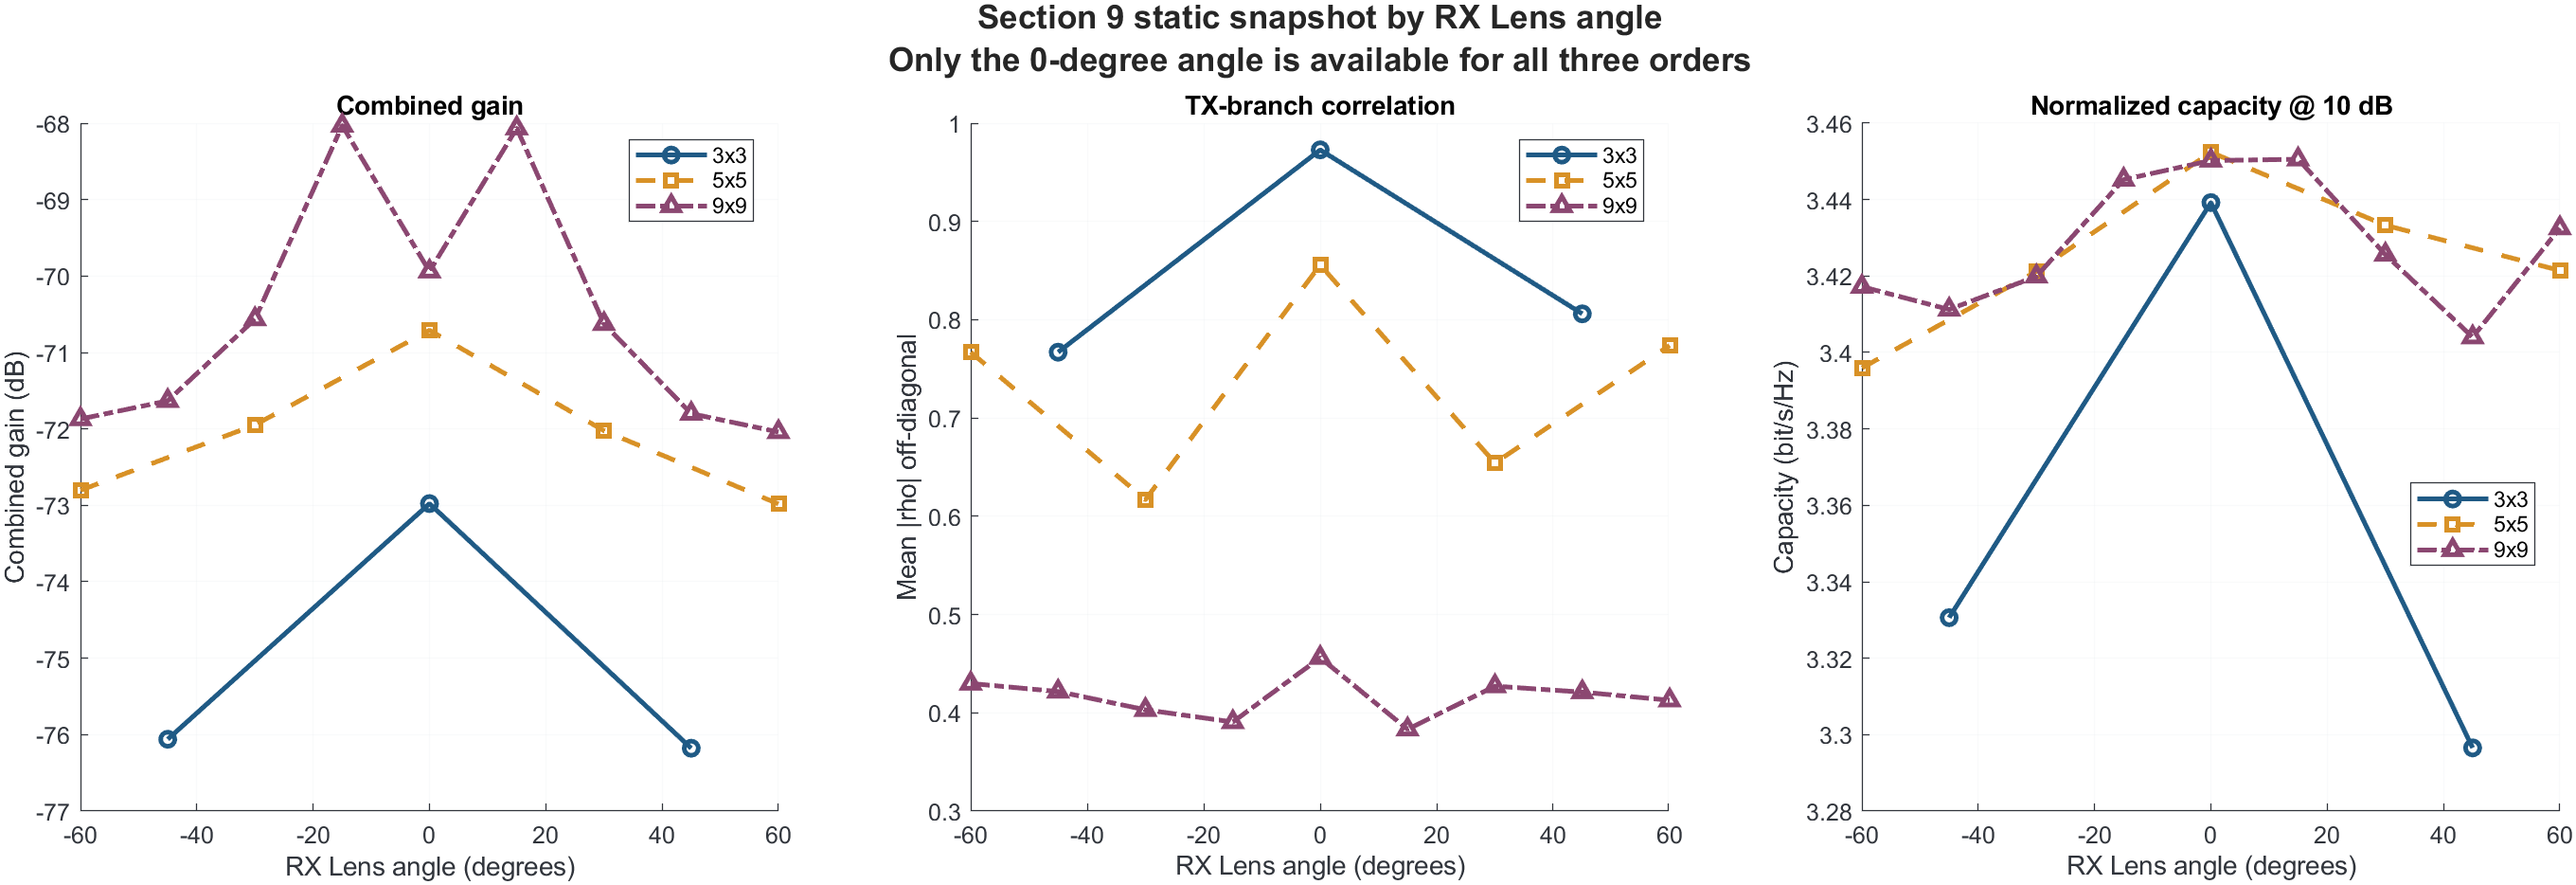
\includegraphics[width=\linewidth]{Images/Analisis_v4_ISO_TX_Lens_Order_3x3_5x5_9x9_Linear/figures_matlab/02_static_rx_by_order_matlab.png}
    \caption{Static combined gain, TX-channel correlation, and normalized per-RX capacity for the three lens-assisted orders. The RX angle grids differ with order.}
    \label{fig:iso-order-static-rx}
\end{figure}

The constructed static matrix does not exhibit a monotonic conditioning trend. As Figure~\ref{fig:iso-order-static-mimo} shows, the condition number is 28.70, 23.40, and 25.10~dB for $N=3$, $5$, and $9$, respectively. The $5\times5$ snapshot also has the largest normalized effective rank (0.666) and capacity per dimension (2.810~bit/s/Hz), compared with 0.533 and 2.413~bit/s/Hz for $N=3$ and 0.569 and 2.653~bit/s/Hz for $N=9$. Meanwhile, mean RX correlation decreases from 0.5636 to 0.2674 as $N$ increases. Thus, the static position suggests favorable angular diversity at higher order, but it cannot represent the complete trajectory.

\begin{figure}[htbp]
    \centering
    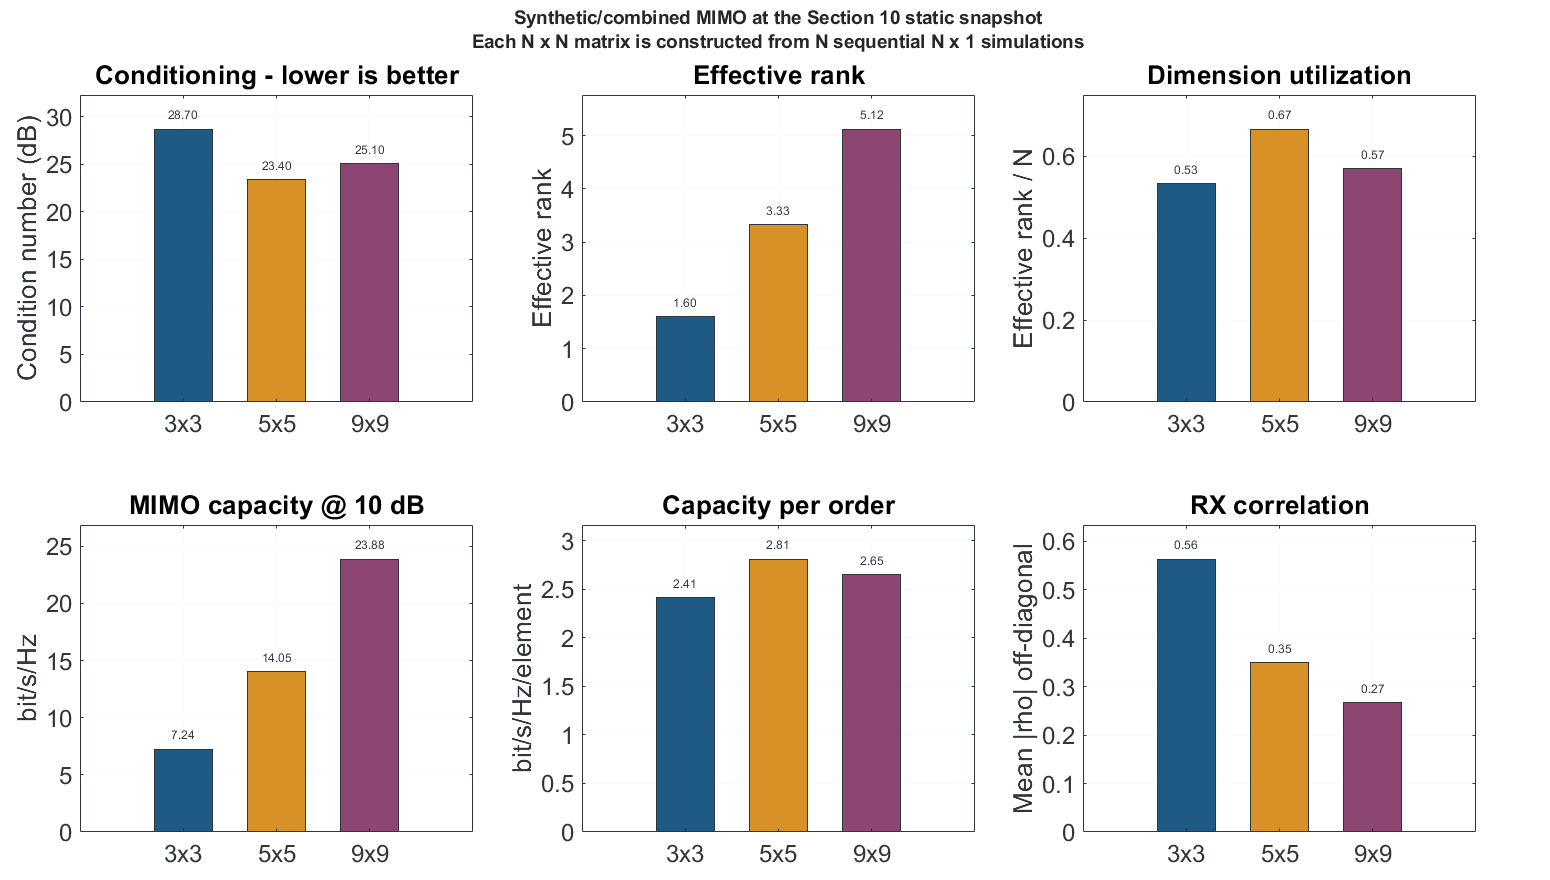
\includegraphics[width=0.98\linewidth]{Images/Analisis_v4_ISO_TX_Lens_Order_3x3_5x5_9x9_Linear/figures_matlab/03_static_mimo_scaling_matlab.png}
    \caption{Constructed static $N\times N$ MIMO metrics versus order. The $5\times5$ configuration is best conditioned and has the highest normalized rank and capacity in this single snapshot.}
    \label{fig:iso-order-static-mimo}
\end{figure}

\subsection{Aggregate and Along-Trajectory Link Scaling}

Table~\ref{tab:iso-order-aggregate-results} and Figure~\ref{fig:iso-order-aggregate} summarize the trajectory results. Median channel magnitude remains within 0.29~dB across the three orders, whereas median link capacity rises from 3.57 to 5.19~bit/s/Hz. The 1.62~bit/s/Hz increase from $N=3$ to $N=9$ corresponds to 45.4\%, but it occurs together with a 4.77~dB increase in nominal total TX power. Outage at the 1~bit/s/Hz threshold is 0\% for every order and is therefore non-discriminating.

\begin{table}[htbp]
    \centering
    \caption{Aggregate link, constructed-MIMO, and spatial-decorrelation metrics along the common linear trajectory. The two capacity metrics are in bit/s/Hz; $D_\mathrm{global}$ and $D_\mathrm{med}$ denote global-pooled and block-median decorrelation, respectively.}
    \label{tab:iso-order-aggregate-results}
    \footnotesize
    \renewcommand{\arraystretch}{1.13}
    \begin{tabularx}{\linewidth}{@{}>{\raggedright\arraybackslash}X *{3}{>{\centering\arraybackslash}p{0.145\linewidth}}@{}}
        \toprule
        \textbf{Metric} & \textbf{$3\times3$} & \textbf{$5\times5$} & \textbf{$9\times9$} \\
        \midrule
        Nominal total TX power (dBm) & 14.77 & 16.99 & 19.54 \\
        Median channel magnitude (dB) & $-86.75$ & $-86.94$ & $-86.65$ \\
        Median link capacity & 3.57 & 4.13 & 5.19 \\
        Median condition number (dB) & 25.55 & 34.24 & 42.88 \\
        Median effective rank & 1.154 & 1.332 & 2.043 \\
        Effective rank fraction, $\eta_r$ & 0.385 & 0.266 & 0.227 \\
        Median MIMO capacity at 10~dB & 5.851 & 8.254 & 14.562 \\
        MIMO capacity per dimension, $\eta_C$ & 1.950 & 1.651 & 1.618 \\
        $D_\mathrm{global}$ & 0.9807 & 0.9276 & 0.8570 \\
        $D_\mathrm{med}$ & 0.5308 & 0.5166 & 0.4876 \\
        \bottomrule
    \end{tabularx}
\end{table}

\clearpage
\begin{figure}[p]
    \centering
    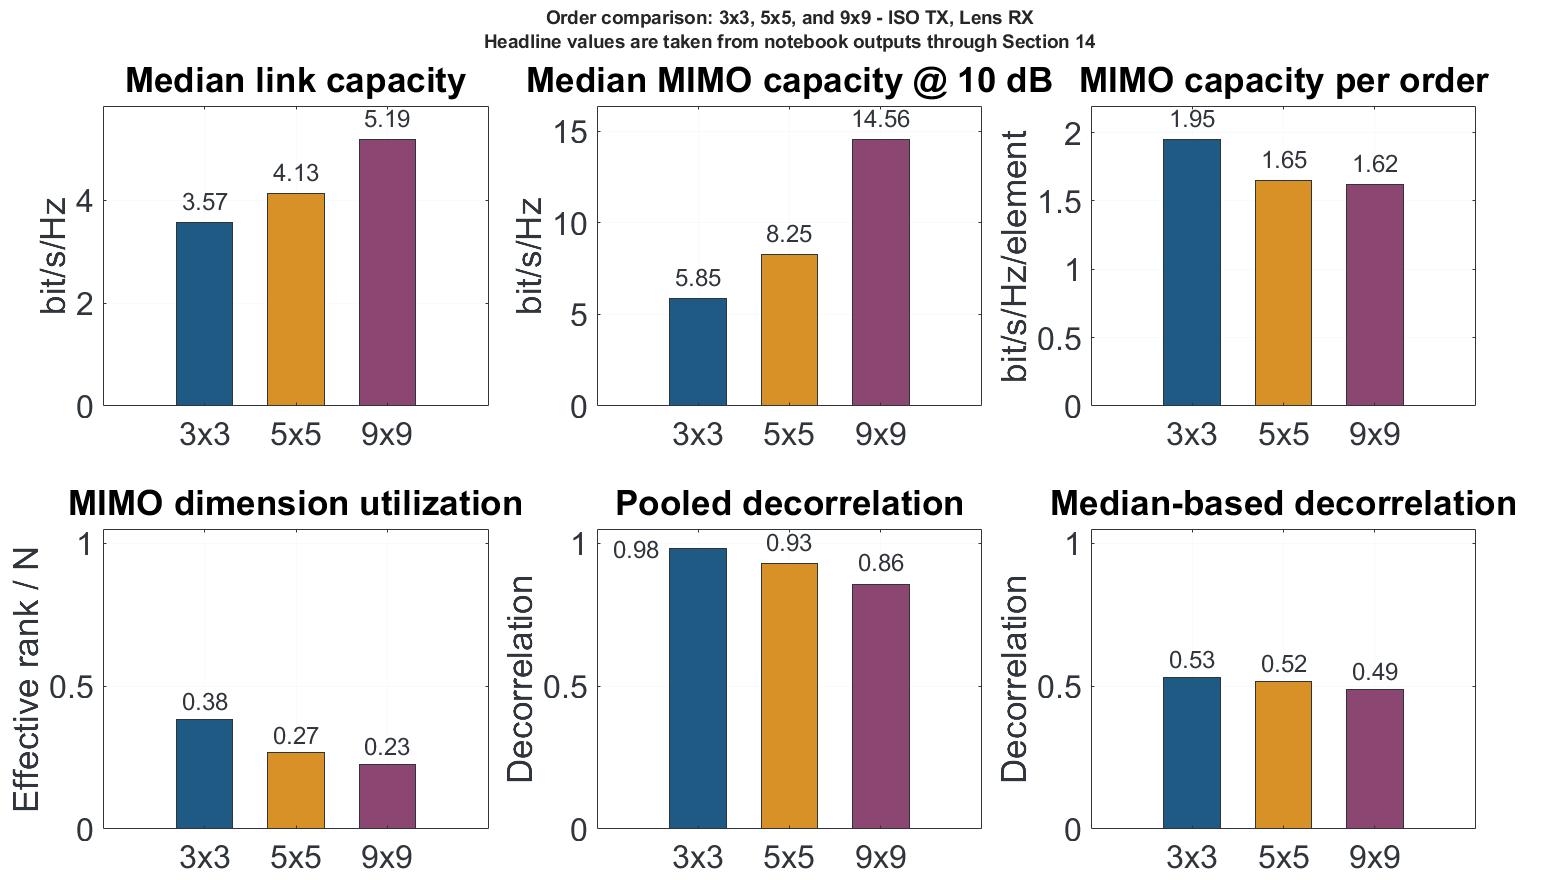
\includegraphics[width=\linewidth]{Images/Analisis_v4_ISO_TX_Lens_Order_3x3_5x5_9x9_Linear/figures_matlab/08_aggregate_order_comparison_matlab.png}
    \caption{Aggregate link, constructed-MIMO, normalized-efficiency, and spatial-decorrelation metrics for the three lens-assisted orders along the common linear trajectory.}
    \label{fig:iso-order-aggregate}
\end{figure}
\clearpage

The common $0^\circ$ RX branch helps separate the changing angular populations, although it does not remove the TX-power and aperture differences. Its median channel magnitude changes from $-86.85$ to $-87.41$~dB between $N=3$ and $N=9$, while SNR rises from 10.70 to 14.96~dB and link capacity from 3.54 to 4.96~bit/s/Hz. The slightly weaker channel response but higher SNR is consistent with the growing aggregate TX power; it does not demonstrate a power-independent order gain.

Figure~\ref{fig:iso-order-link-trajectory} shows the mean channel magnitude and link capacity at each waypoint. The shaded regions are the minimum-to-maximum ranges across the RX branches at a given order, not confidence intervals. Capacity generally rises with order, but the changing band widths and local crossings show that the benefit is dependent on position and lens angle.

\begin{figure}[htbp]
    \centering
    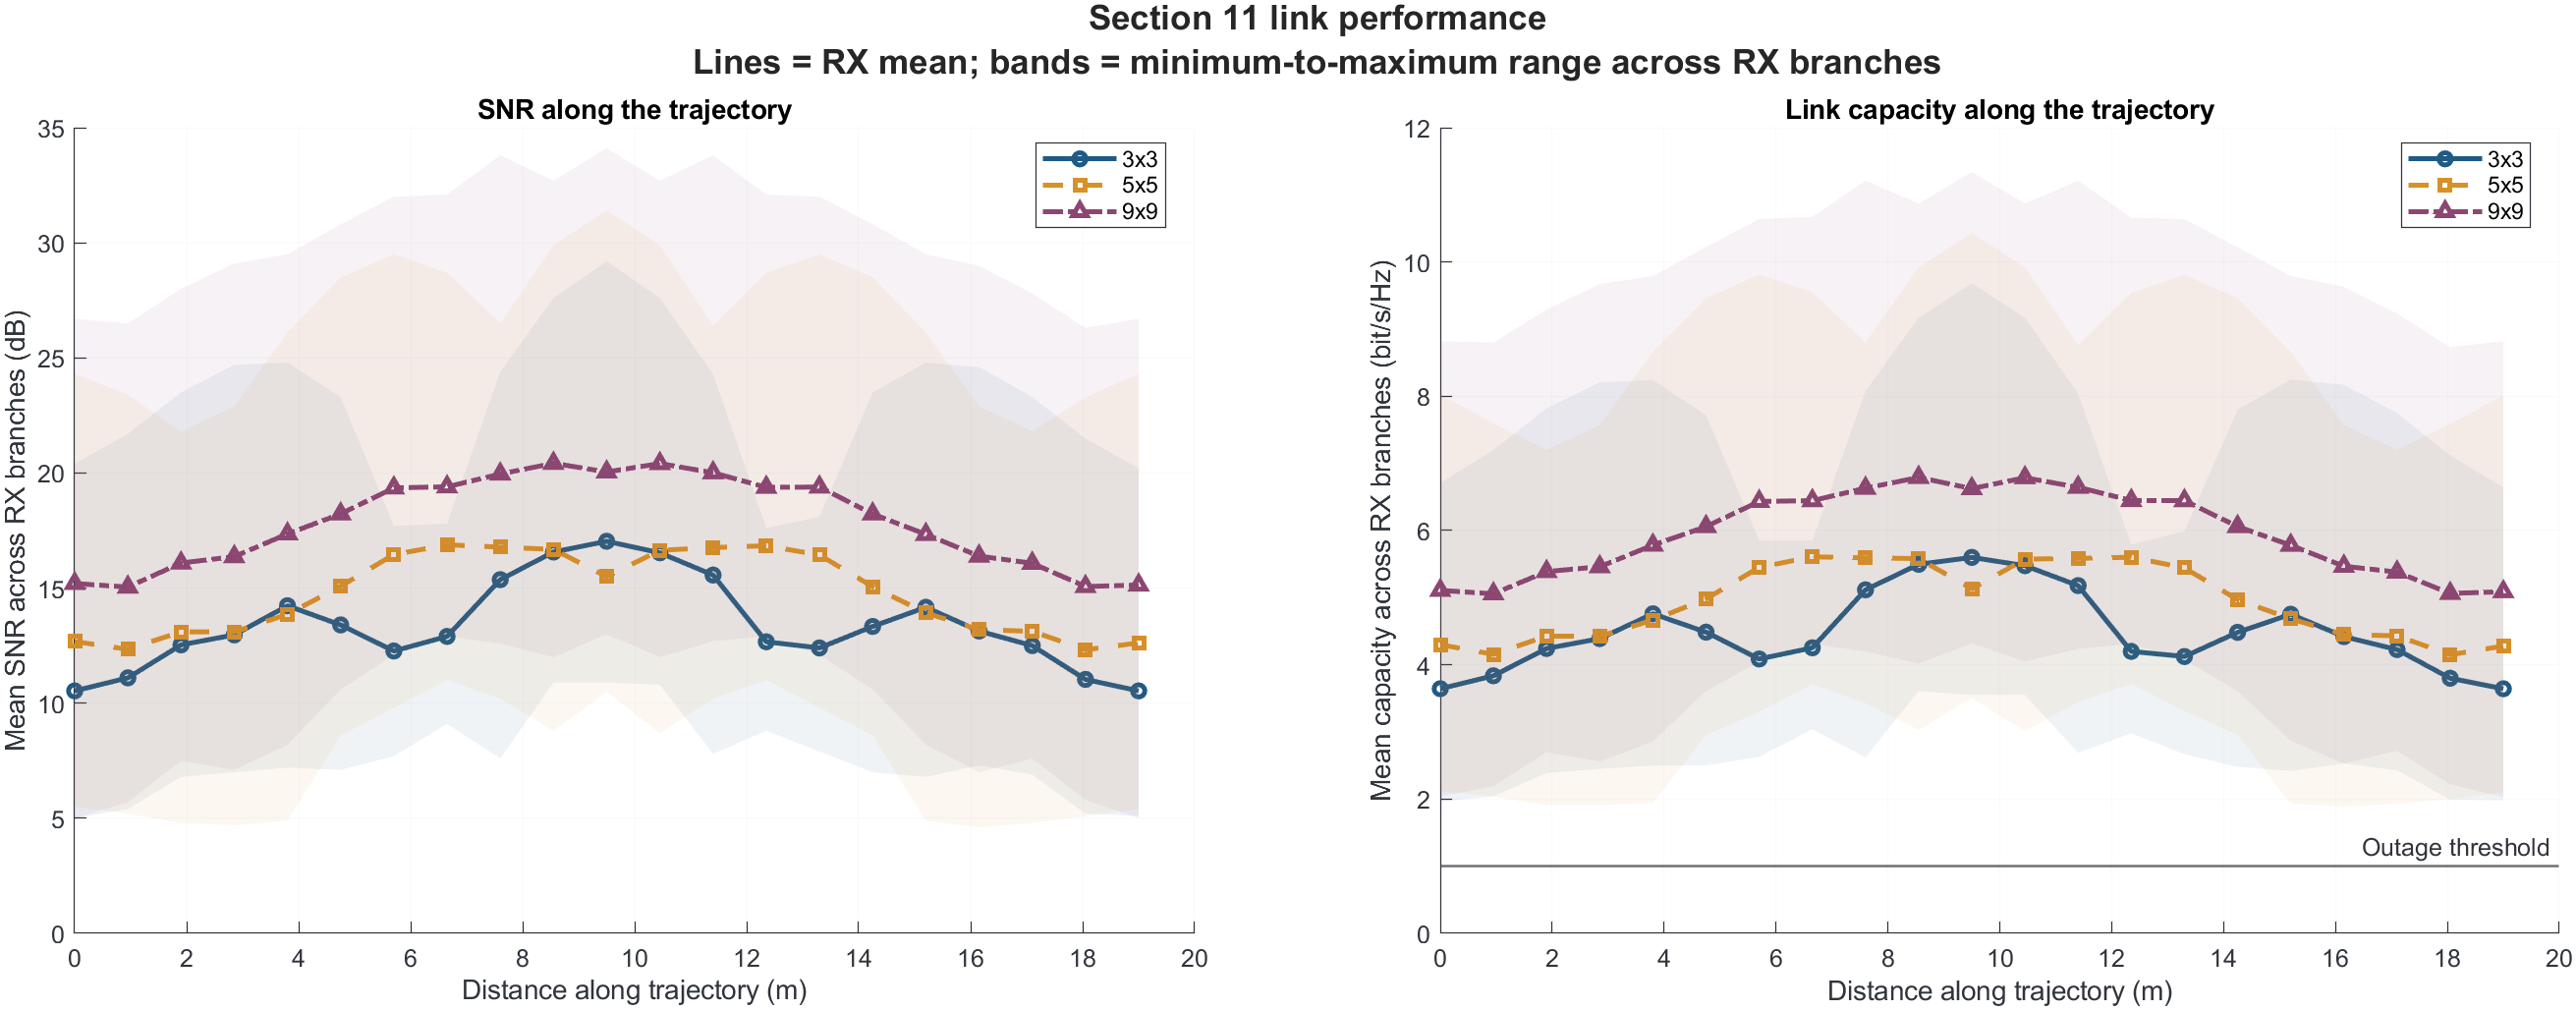
\includegraphics[width=\linewidth]{Images/Analisis_v4_ISO_TX_Lens_Order_3x3_5x5_9x9_Linear/figures_matlab/04_channel_along_trajectory_matlab.png}
    \caption{Mean channel magnitude and link-budget capacity along the common linear trajectory. Shaded regions indicate the minimum-to-maximum range across RX lens branches, not statistical confidence intervals.}
    \label{fig:iso-order-link-trajectory}
\end{figure}

\subsection{Constructed MIMO Scaling Along the Trajectory}

The constructed MIMO capacity increases from 5.851 to 14.562~bit/s/Hz between $N=3$ and $N=9$, an increase of 8.711~bit/s/Hz or approximately 148.9\%. Absolute effective rank also rises from 1.154 to 2.043. These gains are nevertheless sublinear in the number of dimensions. Over the same comparison, effective-rank fraction decreases from 0.385 to 0.227, a relative reduction of approximately 41.0\%, and capacity per dimension decreases from 1.950 to 1.618~bit/s/Hz, or approximately 17.0\%. Median condition number concurrently worsens by 17.33~dB, from 25.55 to 42.88~dB. Higher order therefore adds usable capacity, but the additional dimensions are progressively less balanced and less efficiently utilized.

Figure~\ref{fig:iso-order-mimo-trajectory} also shows a shared bottleneck at the 9.5~m trajectory midpoint. The condition number reaches 55.09, 62.06, and 71.89~dB for $N=3$, $5$, and $9$; effective rank falls to 1.035, 1.061, and 1.085; and MIMO capacity reaches its respective trajectory minimum of 5.185, 6.251, and 7.842~bit/s/Hz. The alignment of the impairment across all orders indicates sensitivity to the common path geometry. It also explains why the non-monotonic static ordering does not persist in the trajectory medians.

\clearpage
\begin{figure}[p]
    \centering
    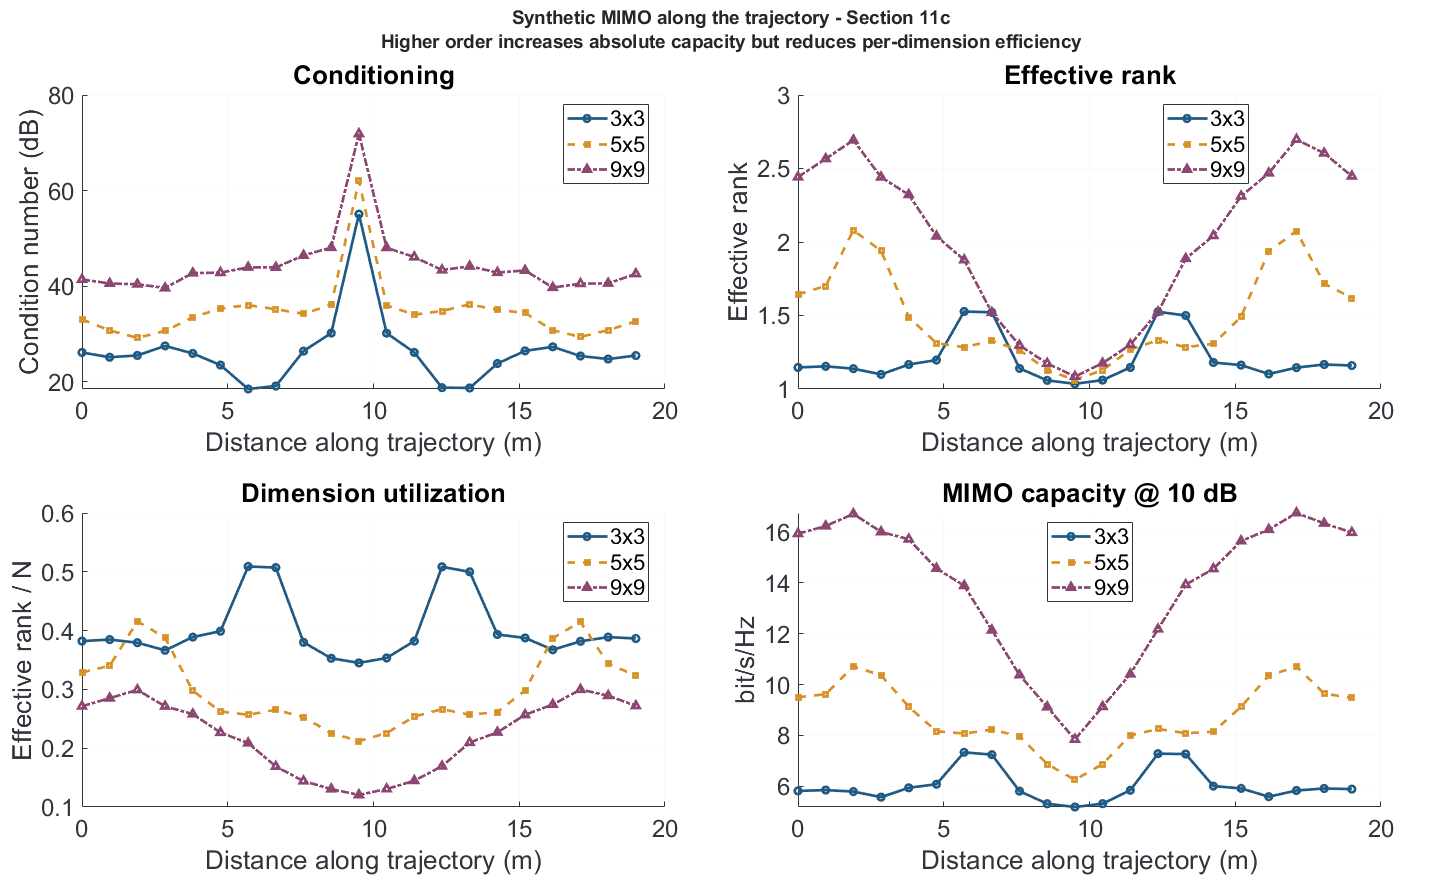
\includegraphics[width=\linewidth]{Images/Analisis_v4_ISO_TX_Lens_Order_3x3_5x5_9x9_Linear/figures_matlab/05_trajectory_mimo_scaling_matlab.png}
    \caption{Condition number, effective rank, normalized effective rank, and ideal MIMO capacity at 10~dB for the constructed $N\times N$ channels along the common trajectory. All orders exhibit a midpoint bottleneck.}
    \label{fig:iso-order-mimo-trajectory}
\end{figure}
\clearpage

\subsection{Spatial Decorrelation Across Orders}

Both aggregate decorrelation estimators decrease monotonically with order. Global pooled decorrelation falls from 0.9807 for $N=3$ to 0.9276 for $N=5$ and 0.8570 for $N=9$. The block-median estimator decreases more modestly, from 0.5308 to 0.5166 and 0.4876. This indicates greater average similarity among the center-TX RX responses in the higher-order configurations under the respective aggregation rules. It does not establish an order-only effect because the RX-pair population grows from 3 to 10 and 36 pairs, and the $9\times9$ grid introduces many closely spaced $15^\circ$ pairs. The number and spacing of RX lens angles therefore change together with $N$.

Figure~\ref{fig:iso-order-decorrelation} presents waypoint-local rather than global-pooled estimates. The mean waypoint-local pooled values are 0.5502, 0.5215, and 0.4934, while the corresponding mean median-based values are 0.5414, 0.5110, and 0.4836. Their overall ordering agrees with the aggregate summary, but the curves cross along the path. Hence, $N=3$ is not more decorrelated at every waypoint, and numerical values from the local curves should not be substituted for the global statistics in Table~\ref{tab:iso-order-aggregate-results}.

\begin{figure}[htbp]
    \centering
    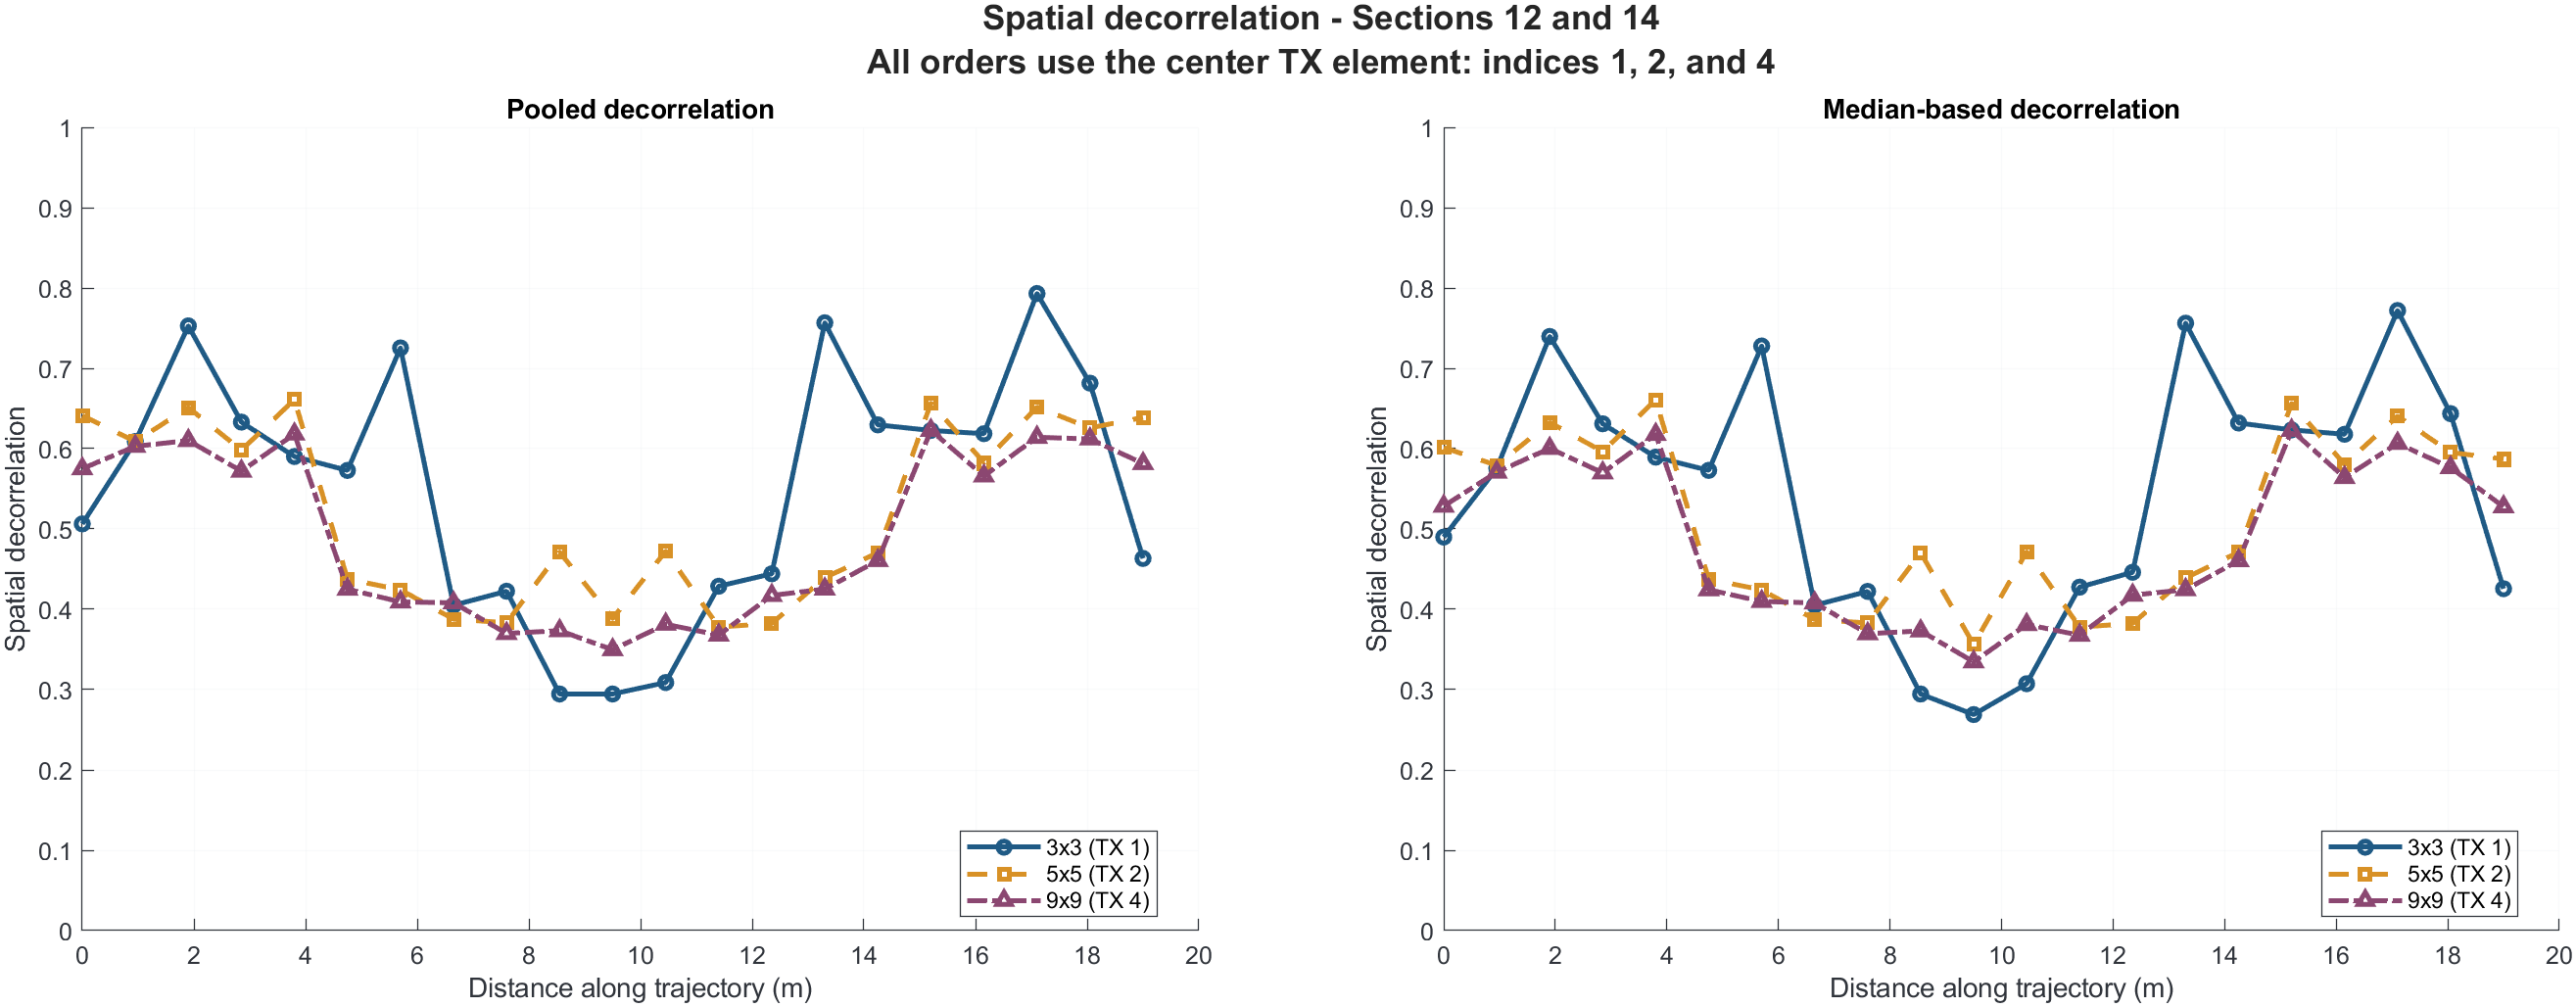
\includegraphics[width=\linewidth]{Images/Analisis_v4_ISO_TX_Lens_Order_3x3_5x5_9x9_Linear/figures_matlab/06_spatial_decorrelation_by_order_matlab.png}
    \caption{Waypoint-local pooled and median-based decorrelation of the center-TX responses across RX lens branches. The curves cross locally even though their trajectory averages decrease with order.}
    \label{fig:iso-order-decorrelation}
\end{figure}

The mean raw difference power in Figure~\ref{fig:iso-order-raw-difference} is non-monotonic: $4.863\times10^{-8}$, $4.205\times10^{-8}$, and $4.628\times10^{-8}$ for $N=3$, $5$, and $9$, respectively. Since this metric preserves path loss and pattern gain, it neither contradicts the normalized decorrelation result nor serves as an independent measure of spatial-channel quality.

\begin{figure}[htbp]
    \centering
    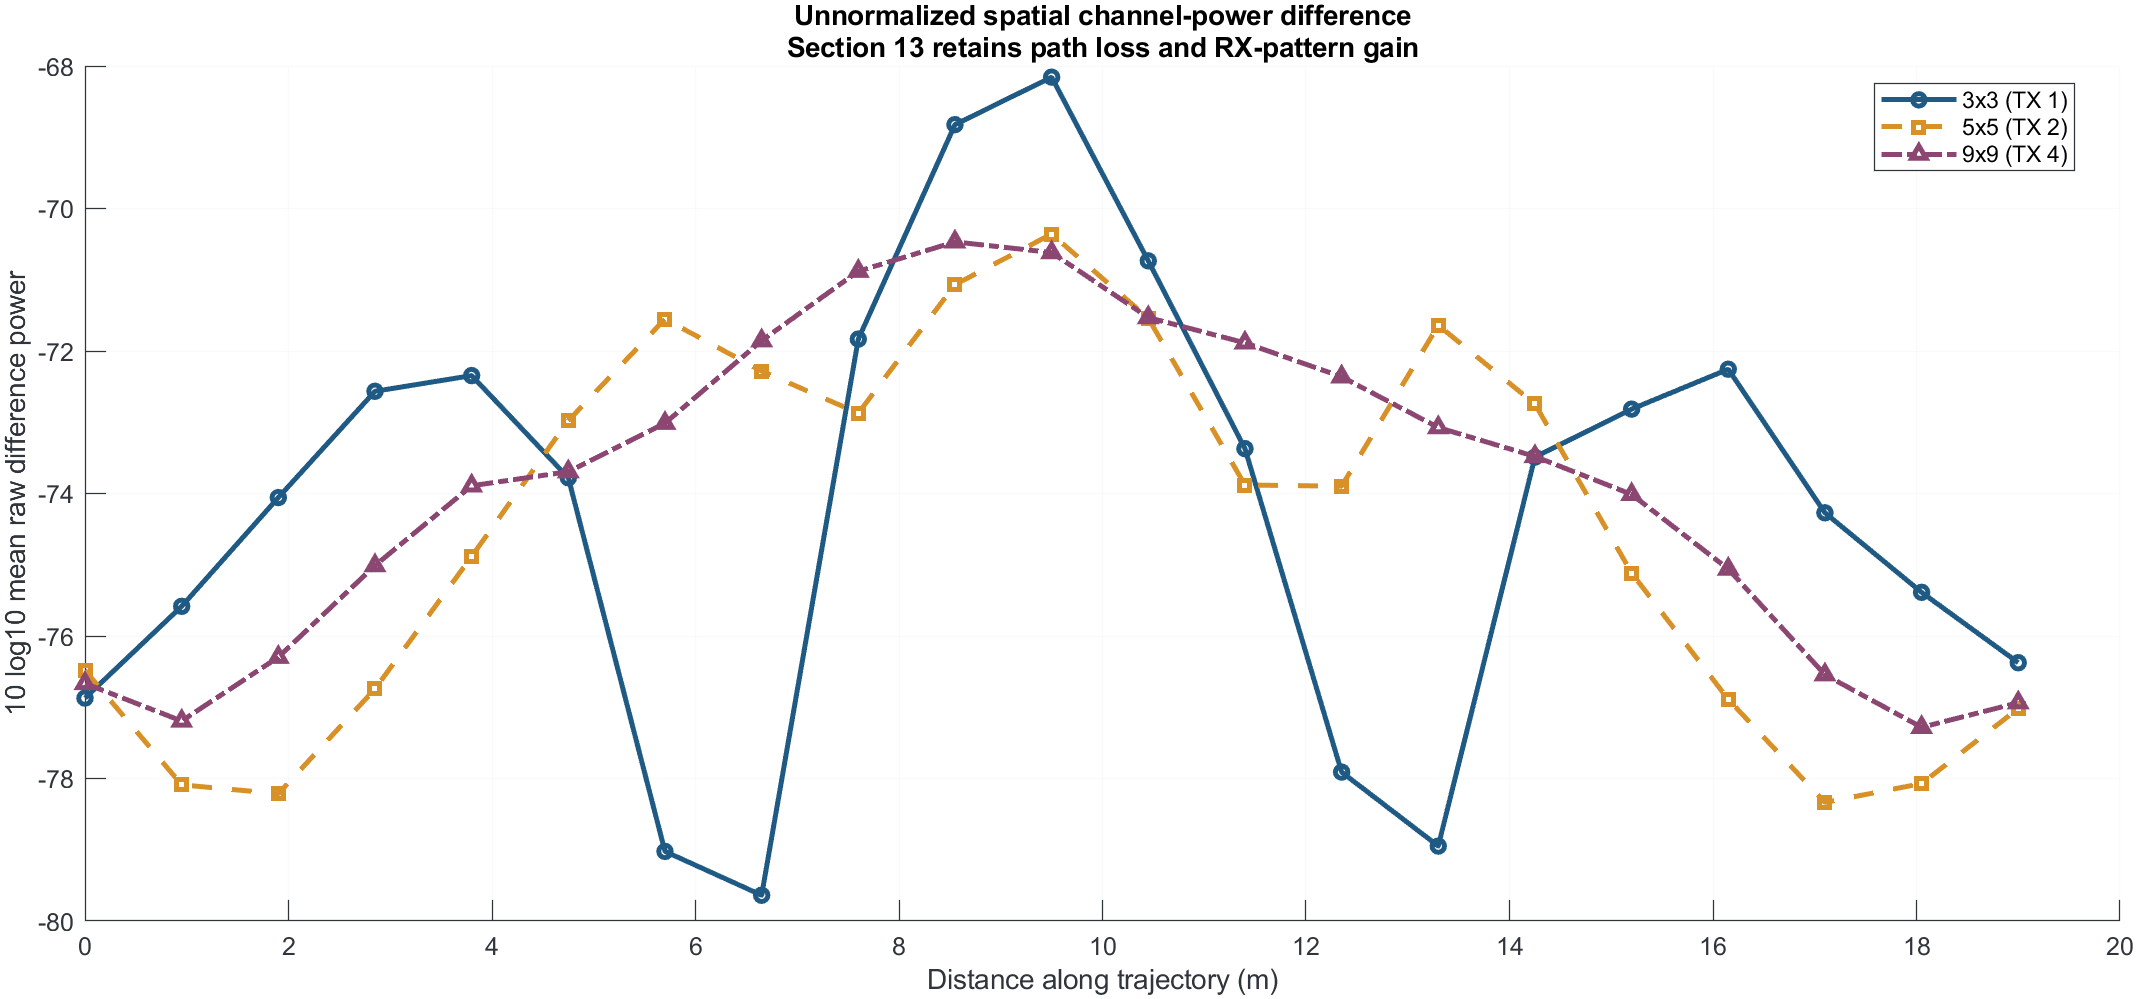
\includegraphics[width=0.95\linewidth]{Images/Analisis_v4_ISO_TX_Lens_Order_3x3_5x5_9x9_Linear/figures_matlab/07_raw_spatial_difference_by_order_matlab.png}
    \caption{Raw center-TX spatial difference power across RX lens branches. The metric is amplitude-sensitive and shows no monotonic order trend.}
    \label{fig:iso-order-raw-difference}
\end{figure}

\subsection{Discussion and Limitations}

The higher-order comparison shows that absolute rate and spatial efficiency answer different design questions. For the link budget, activating more TX elements increases the nominal total radiated power and the reported capacity. Separately, the larger constructed matrix supports a higher absolute MIMO capacity at the same normalized 10~dB SNR. However, the rise in effective rank is much smaller than the rise in $N$, the singular-value spread grows, and both normalized metrics in Equation~\ref{eq:iso-order-normalized-metrics} decrease. Under the evaluated configurations, higher order therefore offers additional aggregate capacity with diminishing utilization of each added spatial dimension.

Position sensitivity is also important. At the static snapshot, $N=5$ has the best condition number and normalized efficiencies, whereas the full-trajectory medians worsen monotonically with $N$. All three configurations experience their worst conditioning and minimum MIMO capacity at the same path midpoint. A single static position can therefore overstate or reverse the order ranking, and higher-order design should be evaluated over its intended motion and orientation distribution.

Several factors prevent causal attribution to $N$ alone. First, 10~dBm is assigned to every TX, so nominal total TX power increases from 14.77 to 19.54~dBm. Second, fixed 0.45~m spacing causes a fourfold aperture increase, and the RX angle grids change in both extent and resolution. Third, only the $0^\circ$ RX branch is common across all orders. Controlled follow-up studies should separately hold total power, aperture, and RX angles constant to quantify their individual contributions.

The channel construction imposes further limitations. Each $N\times N$ matrix stacks $N$ sequential $N\times1$ simulations rather than simultaneous multiport RX measurements; mutual coupling, receiver hardware phase consistency, joint combining, and switching overhead are not represented. The results cover one room, one trajectory, and one stored simulation output without a multi-seed convergence study or confidence intervals. The ray-tracing run uses 100{,}000 path samples per source rather than the 1{,}000{,}000 recommended by the source workflow for a final high-accuracy run. The 1~bit/s/Hz outage threshold is saturated, and the fixed-SNR MIMO capacity is an ideal channel-structure bound rather than coded throughput. Finally, the derived CSV tables and figures pass all 21 packaged validation checks, but the source notebooks referenced by the provenance record are not present in the current archive; the analysis therefore cannot presently be regenerated end to end from the saved notebook outputs.

\subsection{Summary of Higher-Order Scaling}

Along the common lens-assisted linear trajectory, scaling from $3\times3$ to $9\times9$ increases median link capacity from 3.57 to 5.19~bit/s/Hz and constructed-MIMO capacity at 10~dB from 5.851 to 14.562~bit/s/Hz. The gain is not proportional: median condition number worsens by 17.33~dB, effective-rank fraction falls from 0.385 to 0.227, capacity per dimension falls from 1.950 to 1.618~bit/s/Hz, and both aggregate decorrelation estimators decrease. Higher order therefore increases total capacity with diminishing spatial efficiency, but the present results do not establish a power-normalized or aperture-independent advantage.
